\documentclass[12pt,a4paper,titlepage,headinclude,bibtotoc]{scrartcl}

%---- Allgemeine Layout Einstellungen ------------------------------------------

% Für Kopf und Fußzeilen, siehe auch KOMA-Skript Doku
\usepackage[komastyle]{scrpage2}
\pagestyle{plain}
\setheadsepline{0.5pt}[\color{black}]
\automark[section]{chapter}


%Einstellungen für Figuren- und Tabellenbeschriftungen
\setkomafont{captionlabel}{\sffamily\bfseries}
\setcapindent{0em}


%---- Weitere Pakete -----------------------------------------------------------
% Die Pakete sind alle in der TeX Live Distribution enthalten. Wichtige Adressen
% www.ctan.org, www.dante.de

% Sprachunterstützung
\usepackage[ngerman]{babel}

% Benutzung von Umlauten direkt im Text
% entweder "latin1" oder "utf8"
\usepackage[utf8]{inputenc}

% Pakete mit Mathesymbolen und zur Beseitigung von Schwächen der Mathe-Umgebung
\usepackage{latexsym,exscale,stmaryrd,amssymb,amsmath}


\usepackage[nointegrals]{wasysym}
\usepackage{eurosym}

% Anderes Literaturverzeichnisformat
%\usepackage[square,sort&compress]{natbib}
\usepackage{hyperref}
% Für Farbe
\usepackage{color}
\usepackage{graphicx}
\usepackage{wrapfig}
\usepackage{subfigure}

% Caption neben Abbildung
\usepackage{sidecap}

% Befehl für "Entspricht"-Zeichen
\newcommand{\corresponds}{\ensuremath{\mathrel{\widehat{=}}}}
% Befehl für Errorfunction
\newcommand{\erf}[1]{\text{ erf}\ensuremath{\left( #1 \right)}}

%Fußnoten zwingend auf diese Seite setzen
\interfootnotelinepenalty=1000

%Für chemische Formeln (von www.dante.de)
%% Anpassung an LaTeX(2e) von Bernd Raichle
%\makeatletter
%\DeclareRobustCommand{\chemical}[1]{%
  %{\(\m@th
  % \edef\resetfontdimens{\noexpand\)%
   %    \fontdimen16\textfont2=\the\fontdimen16\textfont2
    %   \fontdimen17\textfont2=\the\fontdimen17\textfont2\relax}%
 %  \fontdimen16\textfont2=2.7pt \fontdimen17\textfont2=2.7pt
  % \mathrm{#1}%
  % \resetfontdimens}}
%\makeatother

%Honecker-Kasten mit $$\shadowbox{$xxxx$}$$
\usepackage{fancybox}

%SI-Package
\usepackage{siunitx}

%keine Einrückung, wenn Latex doppelte Leerzeile
\parindent0pt

%Bibliography \bibliography{literatur} und \cite{gerthsen}
%\usepackage{cite}
\usepackage{babelbib}
\selectbiblanguage{ngerman}

\begin{document}

\begin{titlepage}
\centering
\textsc{\Large Praktikum zur Einführung in die physikalische Chemie,\\[1.5ex] Universität Göttingen}

\vspace*{1cm}

\rule{\textwidth}{1pt}\\[0.5cm]
{\huge \bfseries
  V6: Dissoziationskonstante\\[1.5ex]
  einer schwachen Säure}\\[0.5cm]
\rule{\textwidth}{1pt}

\vspace*{1cm}


\begin{Large}
\begin{tabular}{ll}
Durchführende: &  Alea Tokita, Julia Stachowiak\\
Assistentin: & Annemarie Kehl\\
 Versuchsdatum: & 18.01.2016\\
 Datum der 1. Abgabe: & 25.01.2016\\
 Datum der 2. Abgabe: & 04.02.16
\end{tabular}
\end{Large}

\vspace*{1cm}

\large
\begin{table} [h] 
\centering
\begin{tabular} {| p {3 cm}|| p {3 cm}|}
  \hline
  pH & $ K_{\mathrm{s}}$ \\\hline
  $6,2$ & $ (14 \pm 5) \cdot 10^{-8}$\\
  $6,4$& $ (14 \pm 5) \cdot 10^{-8}$\\
  $6,6$& $ (13 \pm 5) \cdot 10^{-8}$\\
  $6,8$& $ (14 \pm 5) \cdot 10^{-8}$\\
  $7,0$& $ (9 \pm 5) \cdot 10^{-8}$\\
  $7,2$& $ (9 \pm 4) \cdot 10^{-8}$\\
  $7,4$& $ (9 \pm 5) \cdot 10^{-8}$\\
  $7,6$& $ (8 \pm 4) \cdot 10^{-8}$\\\hline
  &\\
  Auftragung& $ (15 \pm 5)\cdot 10^{-8}$ \\\hline\hline
  &\\
  Literaturwert (bei $22{~}^\circ$C) & $6,92 \cdot 10^{-8}$\\\hline
 \end{tabular}
\end{table}


\end{titlepage}

\tableofcontents

\newpage

\section{Theoretische Grundlagen}

Die Dissoziationskonstante der schwachen Säure p-Nitrophenol soll mittels Photometrie gemessen werden. \\
Säuren bilden in wässriger Lösung folgendes Gleichgewicht; $\mathrm{A^-}$ beschreibt den Säurerest.\\

\begin{equation}
\mathrm{HA}  \rightleftharpoons \mathrm{H^+} + \mathrm{A^-}
\end{equation}

Die Lage des Gleichgewichtes ist durch das Massenwirkungsgesetz definiert:\\

\begin{equation}
K_\mathrm{c} =\frac{c(\mathrm{H+}*c{A^-}}{c(HA)}
\end{equation}

Der $\mathrm{pK_s}$-Wert ist der negativ dekadische Logarithmus von $\mathrm{K_S}$; der PH-Wert der negativ dekadische Logarithmus der Oxoniumionenkonzentration:

\begin{equation}
\mathrm{p}K_\mathrm{S} = - log_{10} (\frac{c(H^+}{c^0}
\end{equation}

\begin{equation}
\mathrm{PH}= -log_{10}(\frac{c(H^+)}{c^0})
\end{equation}

$c^0$ bezeichnet die Standartkonzentration von 1 $mol\cdot l^{-1}$ und wird verwandt, um den Term einheitenlos zu machen.


Gesucht wird somit nun $\mathrm{c(R^-)}$, da dies für die Abschwächung der Lichtintensität verantwortlich ist. Eine Pufferlösung gibt den PH-Wert vor. Bei Zugabe von einer Säure ändert sich dieser nur schwach und kann mittels der Henderson- Hasselbalch- Gleichung bestimmt werden: \\

%\begin{equation}
%pH = \mathrm{PK_S} + log_{10}\left( \frac{c(A^-}{c(HA)}
%\end{equation}

$\mathrm{c(A^-}$ und $\mathrm{c(HA)}$ beschreibt die Konzentrationen des Puffers im Gleichgewicht. \\

\subsection{Photometrie}
Die Verminderung der Lichtintensität $\mathrm{d}I$ der Lösung im Vergleich zu der Lichtintensität von Wasser $I_0$, ist ein Maß für die Konzentration der absorbierenden Substanz. Sie wird über den Weg $x$, hier gleichzusetzen mit der Küvettenschichtdicke $d$. Sie wird durch das Lambert-Beersche Gesetz beschrieben ergibt die Extinktion $E$:\\

%\begin{equation}
%E = \epsilon _\lambda \cdot c \cdot d = log_{10}\left( %\frac{I_0}{I}
%\end{equation}

$\epsilon_lambda$ beschreibt die Extinktionskonstante. 








\begin{equation}
-\frac{\mathrm{d}I}{\mathrm{d}x} = \alpha \cdot c(A^-) \cdot I
\end{equation}








Henderson-Hasselbalch-Gleichung, Pufferlösung und schwache Säure???








In Lösung bildet p-Nitrophenol folgendes Gleichgewicht:










\begin{center}

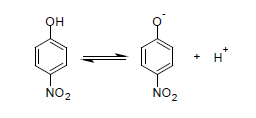
\includegraphics[scale=1]{Strukturformel}

\end{center}
Die dissoziierte und undissoziierte Form weisen eine unterschiedliche Lichtdurchlässigkeit auf.
Bei Auftreffen von Licht klappt die eine Ladung der dissoziierten Form herunter etc. und somit ist die dissoziierte Form gelb und dadurch lichtundurchlässiger als die dissoziierte Form.


\section{Bestimmung der Dissoziationskonstante}




\subsection{Versuchsaufbau}
+ Versuchsaufbau; Photometer

\subsection{Durchführung}





\section{Auswertung}
Im Versuch wird die Messung der Extinktion für jeden pH, sowie für $E_{\infty}$, sechsmal durchgeführt. Anschließend wird daraus für jeden pH der Mittelwert der Extinktion gebildet. Es ergeben sich folgende Mittelwerte:

\begin{table} [h]
\begin{tabular} {| p {1,5 cm}|| p {3 cm}| p{2cm}|}
  \hline
  pH & $\overline{E}$& $E_{\infty}$ \\\hline
  $6,2$& $0,182$&$0,988$\\
  $6,4$& $0,255$&$0,988$\\
  $6,6$& $0,347$&$0,988$\\
  $6,8$& $0,463$&$0,988$\\
  $7,0$& $0,659$&$1,378$\\
  $7,2$& $0,827$&$1,378$\\
  $7,4$& $0,948$&$1,378$\\
  $7,6$& $1,044$&$1,378$\\\hline
 

\end{tabular}
\end{table}

Nun lässt sich $K_{\mathrm{s}}$ folgendermaßen bestimmen:
\begin{align}
K_{\mathrm{s}} = \frac{c(H_3 O^+) \cdot E_\infty}{c^{\circ} \cdot (E_\infty - E_{\mathrm{c}})} = \frac{10^{-pH} \cdot E_\infty}{c^{\circ} \cdot (E_\infty - E_{\mathrm{c}})}
\end{align}

Ebenfalls kann nun $\alpha$ bestimmt werden durch:
\begin{align}
\alpha = \frac{E_{\mathrm{c}}}{E_{\infty}}
\end{align}

Somit ergibt sich:

\begin{table} [h]
\begin{tabular} {| p {1,5 cm}|| p {6 cm}| p{6cm}|}
  \hline
  pH & $K_{\mathrm{s}}$ & $\alpha$ \\\hline
  &&\\
  $6,2$ & 
  $ K_{\mathrm{s}} = \frac{10^{-6,2} \cdot 0,988}{c^{\circ} \cdot (0,988 - 0,182) } = 14,25 \cdot 10^-8 
  $&
  $ \alpha = \dfrac{0,182}{0,988} = 0,184 $ 
  \\
  $6,4$& $13,85\cdot 10^{-8}$& $0,258$ \\
  $6,6$& $13,60\cdot 10^{-8}$& $0,351$\\
  $6,8$& $13,98\cdot 10^{-8}$& $0,468$\\
  $7,0$& $9,015\cdot 10^{-8}$& $0,478$\\
  $7,2$& $9,453\cdot 10^{-8}$& $0,600$\\
  $7,4$& $8,539\cdot 10^{-8}$& $0,788$\\
  $7,6$& $7,579\cdot 10^{-8}$& $0,757$\\\hline
 \end{tabular}
\end{table}

Des weiteren lässt sich $K_{\mathrm{s}}$ aus einer Auftragung bestimmen. Es gilt folgender Zusammenhang, aus welchem sich $K_{\mathrm{s}}$ als Steigung ergibt:
\begin{align}
c(H^+) = (\alpha^{-1} \cdot K_{\mathrm{s}} - K_{\mathrm{s}} ) \cdot c^{\circ} 
\end{align} 

Es muss also $c(H^+)$ gegen $\alpha^{-1}$ aufgetragen werden. Somit ergeben sich für die Auftragung folgende Werte:\\

\begin{table} [h!]
\begin{tabular} {| p {7 cm}| p {7 cm}|}
  \hline
  $c(H^+){~} \mathrm{in} {~}[\mathrm{mol \cdot l^-1}]$ & $\alpha^{-1}$ \\\hline\hline
  &\\
  $c(H^+) = 10^{-pH} = 10^{-6,2} = 63 \cdot 10^{-8}$ & 
  $\alpha^{-1} = \frac{E_{\mathrm{c}}}{E_{\infty}} = \frac{0,182}{0,988} = 5,43$
  \\
  $40 \cdot 10^{-8}$ & $3,88$ \\
  $25\cdot 10^{-8}$& $2,85$\\
  $16\cdot 10^{-8}$& $2,13$\\
  $10\cdot 10^{-8}$& $2,09$\\
  $6,3\cdot 10^{-8}$& $1,67$\\
  $3,4\cdot 10^{-8}$& $1,45$\\
  $2,5\cdot 10^{-8}$& $1,32$\\\hline
 \end{tabular}
\end{table}

Nun lässt sich $K_{\mathrm{s}}$ folgendermaßen bestimmen:
\begin{align}
K_{\mathrm{s}} = \frac{\Delta c(H^+)}{\Delta \alpha^{-1} \cdot c^{\circ}} = \frac{(65-5) \cdot 10^{-8} {~}\mathrm{mol \cdot l^-1}}{(5,5-1,5) \cdot 1 {~}\mathrm{mol \cdot l^-1}} = 15 \cdot 10^{-8}
\end{align}

\newpage

\section{Fehlerrechnung}
\subsection{Fehlerfortpflanzung}
Für die Fehlerfortpflanzung ergibt sich für den pH einen Fehler von $\Delta \mathrm{pH} = 0,1$. Daraus ergibt sich auch der Fehler für $c(H^+)$. Der Fehler für die Extinktion muss als Standardabweichung aus den ermittelten Werten errechnet werden.
Die Standardabweichung des Mittelwerts ergibt sich allgemein aus:
\begin{align}
\overline{S_\mathrm{N}} = \sqrt{\dfrac{1}{\mathrm{N}\cdot (\mathrm{N}-1)} \sum_{\mathrm{i}=1} ^{\mathrm{N}}(x_\mathrm{i}-\overline{x})^2}
\end{align}

Da nur wenige Messungen gemacht werden muss weiterhin der Studentsche Faktor $t_{\mathrm{N}}$ mit einberechnet werden. Für sechs Messungen und ein $95,5\%$ Konfidenzintervall liegt dieser bei $2,6$. Es ergibt sich somit für jeden pH-Wert folgende Standardabweichung:

\begin{table} [h]
\centering
\begin{tabular} {|c|c|c||c|c|c|}
  \hline
  pH & $\overline{S_\mathrm{N}}$ & $\overline{S_\mathrm{N}} \cdot t_{\mathrm{N}} = \Delta E_{\mathrm{c}} $ & $E_{\infty}$ & $\overline{S_\mathrm{N}}$ & $\overline{S_\mathrm{N}} \cdot t_{\mathrm{N}} = \Delta E_{\infty} $ \\\hline\hline
  $6,2$ & $0,00138$& $0,000433$&$E_{\infty {~}\mathrm{pH}{~} 6,2-6,8}$ &$0,000817$ & $0,00212$\\
  $6,4$& $0,000167$& $0,00145$&&& \\
  $6,6$& $0,000558$& $0,00240$&&&\\
  $6,8$& $0,000922$&$0,00120$&&&\\\hline\hline
  $7,0$& $0,0109$& $0,0282$ &$E_{\infty {~}\mathrm{pH}{~} 7,0-7,4}$&$0,00138$& $0,00359$\\
  $7,2$& $0,00567$& $0,0147$&&&\\
  $7,4$& $0,00665$&$0,0173$&&&\\
  $7,6$& $0,00138$&$0,0137$&&&\\\hline
  
 \end{tabular}
\end{table}

So lässt sich nun mithilfe der Gauß`schen Fehlerfortpflanzung für die Dissoziationskonstante zu jedem pH-Wert der absolute Fehler berechnen:

\begin{align}
\Delta K_{\mathrm{s}} = \dfrac{10^{\mathrm{-pH}}}{c^{\circ}(E_{\infty}-E_{\mathrm{c}})} \cdot \sqrt{(\ln (10) \cdot E_{\mathrm{c}} \cdot \Delta \mathrm{pH})^2 + \left(\dfrac{E_{\infty} \cdot \Delta E_{\mathrm{c}}}{E_{\infty}-E_{\mathrm{c}}}\right)^2 + \left(\dfrac{E_{\mathrm{c}} \cdot \Delta E_{\infty}}{E_{\infty}-E_{\mathrm{c}} }\right)^2}
\end{align}
\\
Beispielsweise für den pH $= 6,2$ ergibt sich:\\
\begin{align*}
\Delta K_{\mathrm{s}} = \dfrac{10^{\mathrm{-6,2}}}{0,988-0,182} \cdot \sqrt{(\ln (10) \cdot 0,182 \cdot 0,1)^2 + \left(\dfrac{0,988 \cdot 0,000433 }{0,988-0,182}\right)^2 + \left(\dfrac{0,182 \cdot 0,00212 }{0,988-0,182}\right)^2}
\end{align*}
\vspace{4cm}

Folgende Fehler für jeden pH werden errechnet:
\begin{table} [h]
\begin{tabular} {| p {1,5 cm}|| p {3 cm}|}
  \hline
  pH & $ \Delta K_{\mathrm{s}}$ \\\hline
  $6,2$ & $ 5 \cdot 10^{-8}$\\
  $6,4$& $ 5\cdot 10^{-8}$\\
  $6,6$& $ 5\cdot 10^{-8}$\\
  $6,8$& $ 5\cdot 10^{-8}$\\
  $7,0$& $ 5\cdot 10^{-8}$\\
  $7,2$& $ 4\cdot 10^{-8}$\\
  $7,4$& $ 5\cdot 10^{-8}$\\
  $7,6$& $ 4\cdot 10^{-8}$\\\hline
 \end{tabular}
\end{table}


\subsection{Fehler für die Dissoziationskonstante aus der Auftragung}
Durch das Einzeichen von Grenzgeraden können aus der Auftragung kann die maximale und minimale Steigung bestimmt werden und damit auch der absolute Fehler für $K_{\mathrm{s}}$:
\begin{align}
K_{\mathrm{s{~}min}} = \frac{\Delta c(H^+)}{\Delta \alpha^{-1} \cdot c^{\circ}} = \frac{(50-20) \cdot 10^{-8} {~}\mathrm{mol \cdot l^-1}}{(6,5-1,25) \cdot 1 {~}\mathrm{mol \cdot l^-1}} = 8,9 \cdot 10^{-8}
\end{align} 
\begin{align}
K_{\mathrm{s{~}max}} = \frac{\Delta c(H^+)}{\Delta \alpha^{-1} \cdot c^{\circ}} = \frac{(60-5) \cdot 10^{-8} {~}\mathrm{mol \cdot l^-1}}{(4,5-1,5) \cdot 1 {~}\mathrm{mol \cdot l^-1}} = 18 \cdot 10^{-8}
\end{align}

\begin{align}
\Delta K_{\mathrm{s}} = \dfrac{K_{\mathrm{s{~}max}}-K_{\mathrm{s{~}min}}}{2} = \dfrac{(18-8,9) \cdot 10^{-8}}{2}= 5\cdot 10^{-8}
\end{align}


\newpage
\subsection{Diskussion Systematischer Fehler}
Zusätzlich zu den Fehlern aus der Fehlerfortpflanzung gibt es noch weitere systematische Fehler, welche sich quantitativ nicht erfassen lassen.\\
Die Berechnung von $K_{\mathrm{s}}$ erfolgt über die Konzentration an $\mathrm{H_3 O^+}$-Ionen sowie durch die Bestimmung der Extinktion. Beide Messgrößen können durch systematische Fehler verfälscht werden.\\\\
Die Extinktion wird durch ein Spektralphotometer bestimmt, dabei werden die angesetzten Lösungen verschiedener pH im Wechsel mit reinem Wasser photometriert. Dabei könnte das reine Wasser verunreinigt, oder die Küvette beschmutzt sein. Dies würde im Endeffekt zur Bestimmung einer kleineren Dissoziationskonstante führen. Das verunreinigte Wasser würde das Licht mehr Abschwächen als es sollte, dadurch wäre die Abschwächung der Lichtintensität durch die Lösung im Vergleich dazu nicht so stark sein, was eine schwächere Dissoziation bedeuten würde.\\ Des weiteren ist es möglich, dass bei der Messung mit dem Photometer dieses nicht vollständig geschlossen wurde und ein wenig zusätzliches Licht einfällt. Passiert dies auf der Seite des reinen Wassers würde sich analog zu obiger Überlegung eine größere Dissoziationskonstante ergeben. Geschieht es auf der Seite der Lösung würde der zusätzliche Lichteinfall zur Bestimmung einer kleineren Extinktion und damit auch kleineren Dissoziationskonstante.\\ Dabei ist weiterhin der Fall zu beachten, in dem die Extinktion für $E_{\infty}$ verfälscht wird. Hier würde ein zu großer Wert für die Extinktion einen zu kleinen Wert der Dissoziationskonstante bewirken.\\\\
Des weiteren wird mit der Konzentration an $\mathrm{H_3 O^+}$-Ionen gerechnet. Zur Bestimmung dieser werden Pufferlösungen angesetzt. Bei der Herstellung dieser kann es durch ungenaues Arbeiten zu Fehlern kommen.\\ 
Des weiteren ist p-Nitrophenol eine schwache Säure und eine Veränderung der Konzentration an $\mathrm{H_3 O^+}$-Ionen. Diese ist zwar durch den Puffer sehr gering, wird aber dennoch näherungsweise außer Acht gelassen.\\
Insgesamt kann man sagen, dass bei einer eigentlich höheren Konzentration an $\mathrm{H_3 O^+}$-Ionen die bestimmte Dissoziationskonstante zu klein ist und andersherum.\\\\
     
\newpage
\section{Diskussion}
\subsection{Vergleich mit dem Literaturwerten}
Mit den absoluten Fehlern ergeben sich folgende Werte für $ K_{\mathrm{s}}$:

\begin{table} [h]
\begin{tabular} {| p {1,5 cm}|| p {3 cm}|}
  \hline
  pH & $ K_{\mathrm{s}}$ \\\hline
  $6,2$ & $ (14 \pm 5) \cdot 10^{-8}$\\
  $6,4$& $ (14 \pm 5) \cdot 10^{-8}$\\
  $6,6$& $ (13 \pm 5) \cdot 10^{-8}$\\
  $6,8$& $ (14 \pm 5) \cdot 10^{-8}$\\
  $7,0$& $ (9 \pm 5) \cdot 10^{-8}$\\
  $7,2$& $ (9 \pm 4) \cdot 10^{-8}$\\
  $7,4$& $ (9 \pm 5) \cdot 10^{-8}$\\
  $7,6$& $ (8 \pm 4) \cdot 10^{-8}$\\\hline
 \end{tabular}
\end{table}

Sowie für die Auftragung: $K_{\mathrm{s}} = (15 \pm 5) \cdot 10^{-8} $

Der Literaturwert liegt bei $pK_{\mathrm{s}} = 7,16$ bei $22^{\circ}$C \footnote{https://en.wikipedia.org/wiki/4-Nitrophenol, abgerufen am 24.01.2016} woraus sich der $K_{\mathrm{s}} = 6,92 \cdot 10^{-8}$ ergibt.


\subsection{Disskussion}
Im Vergleich mit den Literaturwerten ist auffällig, das alle Werte eher nach oben abweichen. Die Werte von $ \mathrm{pH} = 7,0- 7,6$ sind näher am Literaturwert und schließen diesen mit ihrem Fehlerintervall ein, während die Werte von $ \mathrm{pH} = 6,2- 6,8$ noch mit dem Fehlerintervall zu groß sind. Der Wert aus der Auftragung weicht am stärksten vom Literaturwert ab. Dies ist dadurch zu erklären, dass beim Zeichnen vor allem die eher fehlerhaften Werte von $ \mathrm{pH} = 6,2- 6,8$ beachtet werden, da die anderen Werte sehr dicht aneinander liegen. Daher wurden bei der Bestimmung der minimalen Steigung vor allem die ersten vier Werte beachtet.\\\\
Die zusätzlichen Abweichungen lassen sich durch systematische Fehler erklären. Da die Werte von unterschiedlichen Photometern gemessen wurden, ist möglicherweise das eine Photometer fehlerhaft. Dies rechtfertigt auch das außer Acht lassen der Werte in der Bestimmung des minimalen Wertes für $K_{\mathrm{s}}$. Des weiteren  kann wie bereits erläutert eine Abweichung der Werte nach oben durch Lichteinfall auf der Seite des reinen Wassers, Lichteinfall beim Messen von $E_{\infty}$, oder Ungenauigkeiten beim Herstellen der Pufferlösungen, sowie die dabei durchgeführten Näherungen entstehen.\\\\
Zur Verbesserung des Versuchs könnten zunächst letztere Ungenauigkeiten durch den Gebrauch von größeren Pipetten vermieden werden. Da nämlich die benutzen Pipetten lediglich $10{~} \mathrm{ml}$ umfassten musste die Lösung in mehreren Teilschritten angesetzt werden, was relativ fehleranfällig ist. Des weiteren müssten die Messungen häufiger durchgeführt werden, außerdem auch mit jeweils einem neuen Teil der Lösungen.
 
\newpage
\subsection{Literaturverzeichnis}
https://en.wikipedia.org/wiki/4-Nitrophenol, abgerufen am \textbf{24.01.2016}

\end{document}
